\chapter{NP-Komplethedsbeviser}

\section{Tidskompleksitet}%
\label{subsec:label}

\begin{definition}
	Lad $M$ være en Deterministisk Turingmaskine som stopper på alle inputs. \textit{Køretiden} eller \textit{tidskompleksiteten} af $M$ er funktionen $f : \mathbb{N} \rightarrow \mathbb{N}$, hvor $f(n)$ er maksimum antal af skridt som $M$ tager på ethvert input af længde $n$.
\end{definition}

Altså hvis køretiden for eksempel er $3n^{2}$ betyder det at $M$ vil tage højest $3n^{2}$ skridt hvor længden af inputtet er $n$.

\begin{definition}
	Lad $f,g : \mathbb{N} \rightarrow \mathbb{R}^{+}$ være funktioner. Vi siger at $f(n) \in O(g(n))$ hvis der eksisterer $c, n_{0} \in \mathbb{Z}_{+}$ således at $\forall n \ge n_{0} : f(n) \le c \cdot g(n)$
\end{definition}

Intuitivt betyder det at $f(n)$ er mindre end eller lig med $O(g(n))$.

\begin{definition}
	Lad $f, g  \in \mathbb{N}  \rightarrow \mathbb{R}^{+}$. Vi siger at $f(n) \in o(g(n))$ hvis $\lim_{n \to \infty} \frac{f(n)}{g(n)} = 0$. Altså, for hvert $c > 0$ eksisterer der et $n_{0} = n_{0}(c)$ hvor $\forall n \ge n_{0} $ $f(n)  < cg(n)$.
\end{definition}

Intuitivt betyder det at $f(n)$ gror meget langsommere end $o(g(n))$.

\begin{definition}
	Lad $t : \mathbb{N} \rightarrow \mathbb{R}^{+}$ være en funktion. Lad tidskompleksitetsklassen \textit{TIME($t(n)$)} være samlingen af alle sprog som er afgørlige i tid $O(t(n))$ af en Deterministisk Turingmaskine.
\end{definition}

Det er vigtigt at bemærke at \textit{TIME($t(n)$)} kun omhandler afgørselsproblemer, altså problemer hvor man kan svare ``Ja'' eller ``Nej'' til, og ikke problemer såsom sortering.

Hvis et problem har både en optimisering og af afgørselsversion, så er kompleksiteten af dem tæt relateret. For eksempel ved Spanning Tree er der Minimum Spanning Tree problemet, som søger at finder et minimumsstørrelses spanning tree. Dog er der også en afgørselsversion der spørger om der er et spanning tree med vægt $\le k$.

Givet $G = ( V,E,w )$ og $k \in \mathbb{N}$  kan vi afgøre om $\langle G , k \rangle $ er et spanning tree med vægt højest $k$ ved at løse minimum spanning ree problemet på $\langle G \rangle $ og sammenligne $w(T^{*})$ med $k$. Dermed $\langle G, k \rangle \in SpT_{k} \iff w(T^{*}) \le k$, hvor $T^{*}$ er et minimum spanning tree af $G$ med vægtfunktion $w$.

Hvis vi kun har en algoritme til at løse afgørselsversionen, kan vi finde optimeringsversionen ved at lade $k$ være minimumsværdien (normalvist 1), og så gå op derfra, altså prøve med $k$ indtil der er en success. Hvis $i-1$ ikke findes, men $i$ gør, så ved vi at $i$ er minimum.

\begin{definition}
	Lad $M$ være en nondeterministisk Turingmaskine som er en afgører. \textit{Køretiden} af $M$ er funktionen $f : \mathbb{N} \rightarrow \mathbb{N}$ hvor $f(n)$ er maksimumsantallet af skridt som $M$ bruger på en gren af dens komputering på et input af længde $n$.
\end{definition}

Det vil altså sige, at det er den gren der går længst ned, hvor, ved en deterministisk Turingmaskine, er det blot den enkelte gren den har til rådighed.

\begin{theorem}
	Lad $t(n)$ være en funktion hvor $t(n) \ge n$. Så har hver $t(n)$-tids Nondeterministisk Turingmaskine en ækvivalent $w^{O(t(n))}$-tids enkeltbånds Turingmaskine.
\end{theorem}

\begin{proof}
	Vi beviste dette tidligere MANGLER
\end{proof}

Alle \textit{rimelige} deterministiske komputeringsmodeller er polynomielt ækvivalente. Det vil altså sige at alle varianter af Turingmaskiner kan konverteres til hinanden i polynomiel tid, og køre i polynomiel tid.

\subsection{Klassen $\mathcal{P}$}%
\label{subsec:label}

\begin{definition}
	Klassen $\mathcal{P}$ er kompleksitetsklassen af alle problemer der kan løses af Deterministiske Turingmaskiner i polynomiel tid.
	\begin{equation}
		\mathcal{P} = \bigcup_k TIME(n^{k})
	\end{equation}
\end{definition}

Man kan tænke på $\mathcal{P}$ som værende klassen af problemer der realistisk set kan løses af en moderne computer.

Når vi laver en kodning af et problem, skal vi ikke bruge unær notation (altså base-1), da dette er eksponentielt større end alle base-$k$, hvor $k \ge 2$.


Følgende er nogle eksempler på problemer der er en del af kompleksitetsklassen $\mathcal{P}$:
\begin{enumerate}
	\item $S_{p}T_{k}$ som var afgørlighedsversionen af $MST$.
	\item $PATH = \{\langle G , s, t \rangle \mid G \text{ er en rettet graf } s, t, \in V(G) \text{ og } \exists (s,t) \text{ vej i } G\}$
	\item Medlemskab af kontekstfrie sprog: $CFL\text{-}MEMBER = \{\langle G , w \rangle \mid G \text{ er en CFG og } w \in L(G)\}$
	      \begin{enumerate}
		      \item Givet $w \in \Sigma^{*}$ og $G$ som en Chomsky Grammatik, ved vi at $S \stackrel{*}{\Rightarrow} w$ $\iff$ der er en afledning på $2|w| - 1$ skridt.
		      \item Vi ved det er afgørligt, da vi bare kan prøve alle $2|w|-1$ afledeninger. Dette er dog ikke polynomielt i $|w|$.
	      \end{enumerate}
\end{enumerate}

Vi vil gerne kigge videre på problemet om CFL-medlemskab. Vi kan gøre dette polynomielt, men ikke med en naiv metode. I stedet bruger vi \textit{dynamisk programmering}.

Hvis vi antager at $w = \varepsilon$, så kan vi acceptere hvis $S \rightarrow \varepsilon$ er i $R$. Vi kan derfor antage at $|w| > 0$, og at vi kan sætte $w$ op således: $w = a_{1}a_{2} \ldots a_{n}$. $n = |w|$ $a_{i} \in \Sigma$.

Vi konstruerer en $n \times n $ matrix $T$, hvor $T_{ij} = \{A \mid A \Rightarrow a_{i}a_{i+1} \ldots a_{j}\}$ efter komputering. Til at starte med er $T_{ii} = \{A \mid A \rightarrow a_{i} \in R\}$. Vi bruger følgende idé: Hvis $A \rightarrow BC$ og $B \Rightarrow a_{i} \ldots a_{j}$ og $C \Rightarrow a_{j+1} \ldots a_{p}$, så tilføjer vi $A$ til $T_{ip}$. Det betyder så at når vi er færdige med at køre algoritmen, hvis $T_{1n}$  indholder symbolet $S$ kan vi svare ``Ja'' givet en instans, og ellers ``Nej''.

\begin{algorithm}
	\caption{\label{alg:dynamiccfl}Dynamisk Programmerings CFL Løsning}
	\begin{algorithmic}[1]
		\FOR{$i \gets 1$ \TO $n$}
		\FOR{$j \gets i$ \TO $n$}
		\STATE $T_{ij} \gets \emptyset$
		\ENDFOR
		\ENDFOR

		\FOR{$i \gets 1$ \TO $n$}
		\STATE $T_{ii} \gets \{ A \mid A \to a_i \in R \}$
		\ENDFOR

		\FOR{$r \gets 1$ \TO $n-1$}
		\FOR{$i \gets 1$ \TO $n-r$}
		\FOR{$k \gets i$ \TO $i+r-1$}
		\FORALL{rule $A \to BC$}
		\IF{$B \in T_{ik}$ \AND $C \in T_{k+1,i+r}$}
		\STATE $T_{i,i+r} \gets T_{i,i+r} \cup \{ A \}$
		\ENDIF
		\ENDFOR
		\ENDFOR
		\ENDFOR
		\ENDFOR

		\IF{$S \in T_{1n}$}
		\STATE accepter
		\ELSE
		\STATE afvis
		\ENDIF
	\end{algorithmic}
\end{algorithm}

I Algoritme~\ref{alg:dynamiccfl} ses algoritmen beskrevet over.

\begin{definition}
	En \textit{verifikator} for et sprog $L$ er en algoritme $A_{L}$ hvor \\$L = \{w \mid \exists \text{ en streng } c \text{ hvor } A_{L} \text{ accepterer input } \langle w, c \rangle \}$
\end{definition}

Køretiden af $A_{L}$ måles i form af $n = |w|$. $A_{L}$ er en polynomiel verifikator hvis den har køretid $O(n^{k})$. Strengen 4c = c(w) er et \textit{certifikat} for $w \in L$. Bemærk at $|c(w)| \le $ køretiden af $A_{L}$.

For eksempel ved hamiltoniansk kreds problemet, er en verifikator en der tjekker om, givet et certifikat som indeholder en ordning af knuder, om disse knuder former en kreds, og om kardinaliteten af certifikatet er lig med antallet af knuder.

\begin{definition}
	Kompleksitetsklassen $\mathcal{NP}$ er klassen hvor problemerne har en verifikator som kører i polynomiel tid:
	\begin{equation}
		\mathcal{NP} = \{ L \mid L \text{ er en verifikator der kører i polynomiel tid}\}
	\end{equation}
\end{definition}

Bemærk dog at $\mathcal{NP}$ originalt står får \textit{Nondeterministisk Polynomielt}. Vi kigger på eksempel ved \textit{Hampath} som er en vej der går gennem alle knuder, og ser hvordan den kan konstrueres af en nondeterministisk Turingmaskine. Husk at ved en vej i en graf er $s$ startknuden og $t$ slutknuden.

\begin{enumerate}
	\item Gæt $n$ tal $i_{1}, i_{2}, \ldots, i_{n}$ hvor $i_{j} \in \{1, \ldots, n\}$
	\item Tjek om der er nogle ens lister ($i_{p} = i_{q}, p \ne q$). Hvis ``Ja'', \textit{afvis} denne gren.
	\item Tjek om $s = v_{i_{1}}$ og om $t = v_{i_{n}}$. Hvis ``Nej'', \textit{afvis} denne gren.
	\item Tjek om $(v_{i_{p}},v_{i_{p+1}})$ er en kant for $p = 1,2, \ldots, n-1$. Hvis ``Ja'' \textit{accepter}, ellers \textit{afvis}.
\end{enumerate}

\begin{theorem}
	\begin{equation}
		L \in NP \iff L \text{ kan afgøres af en nondeterministisk Turingmaskine}
	\end{equation}
\end{theorem}

\begin{proof}
	Lad $L \in NP$ og $A_{L}$ være en \textit{verifikator} for $L$ hvor $A_{L}$ kører i højest $dn^{k}$ tid, for en konstant $d$ på input af længde $n$.

	Den nondeterministiske Turingmaskine kører som følger:
	\begin{enumerate}
		\item Vælg nondeterministisk en streng $c$ således at $|c| \le dn^{k}$
		\item Kør $A_{L}$ på \(\langle w, c \rangle \)
		\item Accepter hvis $A_{L}$ accepterer, ellers \textit{afvis}.
	\end{enumerate}

	Omvendt, antag at $L$ er afgjort af en nondeterministisk Turingmaskine $M$. Vi konstruerer $A_{M}$ på input \(\langle w, c \rangle \):
	\begin{enumerate}
		\item Simulér $M$ på \(\langle w \rangle  \) ved at bruge \( \langle c \rangle \) til at guide os til hvilken gren vi skal bruge.
		\item Hvis denne gren af $M$'s komputering resulterer i $M$ som accepterer $w$, så accepterer $A_{M}$ \(\langle w , c \rangle \), ellers \textit{afvis}.
	\end{enumerate}

	Altså eksisterer der et $c$ hvor $A_{M}$ accepterer \( \langle w , c \rangle \) $\iff$ $M$ accepterer $\langle w \rangle $.
\end{proof}

\section{Polynomielle Reduktioner}%
\label{sec:label}

\begin{definition}
	Lad $A, B$ være sprog over alfabetet \(\Sigma\). En \textit{polynomiel reduktion} fra $A$ til $B$ er en funktion $f : \Sigma^{*} \rightarrow \Sigma^{*}$ således at:
	\begin{enumerate}
		\item $x \in A \iff f(x) \in B$
		\item Der eksisterer et positivt heltal $k = k(A,B)$ hvor $f(x)$ kan udregnes i $O(|x|^{k})$ tid.
	\end{enumerate}
	Hvis en sådan funktion eksisterer, skriver vi $A \le_{p} B$.
\end{definition}

Definitionen på \textit{polynomielle reduktioner} minder meget om \textit{mapping reduktioner} fra beregnelighedsdelen af kurset. Der er dog én meget vigtig forskel: Vi må kun bruge \textit{polynomiel tid} til at udregne funktionen $f$.

\begin{lemma}
	Hvis $A \le_{p} B$ og $B \in \mathcal{P}$ så $A \in \mathcal{P}$.
\end{lemma}

\begin{proof}
	Antag at $A_{B}$ afgører $B$ i tid $O(n^{c})$ og $C_{A \rightarrow B}$ beregner $f$ således atg $x \in A \iff f(x) \in B$ i tid $O(n^{k})$

	\begin{center}
		\begin{tikzpicture}[auto, thick, node distance=2.5cm, >=triangle 60]
			% Nodes
			\node (alpha) at (0,0) {$\alpha$};
			\node (q0) [right of=alpha] {$f(x)$};
			\node (f) [right of=q0] {};
			\node (acc) [right=-0.3cm of f] {\{accept, afvis\}};

			% Labels
			\path[->] (alpha) edge[bend left] node {$C_{A \to B}$} (q0);
			\path[->] (q0) edge[bend left] node {$\mathcal{A}_B$} (f);

		\end{tikzpicture}
	\end{center}

	Altså betyder det at $C_{A \rightarrow B}$ udregner $f$ i tid $O(n^{k})$ og dermed, hvis input $x$ har størrelse $n = |x|$, og $A_{B}$ udregner i $O(n^{c})$ så får vi en algoritme der kører i $O(n^{c})$ køretid på et input af størrelse $|f(x)| \in O(n^{k})$. Altså producerer $A_{B}$ et svar i tid $O(|f(x)|^{c}) = O((n^{k})^{c}) = O(n^{ck})$
\end{proof}

\begin{definition}
	Et sprog $L$ kaldes \textit{$\mathcal{NP}$-Komplet} hvis
	\begin{enumerate}
		\item $L \in \mathcal{NP}$
		\item \(\forall L' \in \mathcal{NP} : L' \le_{p}\)
	\end{enumerate}
\end{definition}

$\mathcal{NP}$-Komplethedsklassen eksisterer udelukkende grundet \textit{Cook-Levin} sætningen, som vi kommer til senere (Kapitel~\ref{chap:cooklevin}). Vi skriver $L \in \mathcal{NPC}$ hvis $L$ er $\mathcal{NP}$-komplet.

\begin{theorem}
	Hvis $L \in \mathcal{NPC}$ og $L \le_{p} \hat{L}$ så $\hat{L} \in \mathcal{NPC}$.
\end{theorem}
\begin{proof}
	Vi viser først grafisk:

	\begin{center}
		\begin{tikzpicture}[auto, thick, node distance=2.5cm, >=triangle 60]
			% Nodes
			\node (alpha) at (0,0) {$L'$};
			\node (q0) [right of=alpha] {$L$};
			\node (f) [right of=q0] {$\hat{L}$};
			\node (one) [gray] at (0,-0.5) {$x$};
			\node (two) [gray, right of=one] {$f(x)$};
			\node (three) [gray, right of=two] {$g(f(x))$};

			\node (time) [TurquoiseGreen] at (1.3, 0) {$O(n^{r})$};
			\node (time) [TurquoiseGreen] at (3.8, 0) {$O(n^{s})$};

			% Labels
			\path[->] (alpha) edge[bend left] node {$f$} (q0);
			\path[->] (q0) edge[bend left] node {$g$} (f);

		\end{tikzpicture}
	\end{center}
	\begin{center}
		\begin{tikzpicture}[auto, thick, node distance=2.5cm, >=triangle 60]
			% Nodes
			\node (alpha) at (0,0) {$x$};
			\node (q0) [right of=alpha] {$g(f(x))$};
			\node (test) [TurquoiseGreen] at (1.0,0) {$O(n^{rs})$};

			% Labels
			\path[->] (alpha) edge[bend left] node {$g \circ f$} (q0);

		\end{tikzpicture}
	\end{center}

	Vi laver altså en reduktion hvor vi først reducerer fra $L'$ til $L$ i tid $O(n^{r})$. Dette producerer et nyt output fra $x$, kaldet $f(x)$, givet en funktion $f$. Derefter reducerer vi fra $L$ til $\hat{L}$ i tid $O(n^{s})$, hvilket giver et nyt output fra $f(x)$ kaldet $g(f(x))$ givet en funktion $g$. Hvis vi sætter disse to tider sammen, får vi en reduktion i tid $O(n^{rs})$. Dette betyder at $x \in L' \iff g(f(x)) \in \hat{L}$. Dermed, $L' \le_{p} \hat{L} \; \forall L' \in \mathcal{NP}$.
\end{proof}


\subsection{Satisfiability}%
\label{subsec:label}

\begin{definition}
	En \textit{boolsk variabel} $x$ tager to værdier: \textit{Sand og Falsk} (T, F). Nogle gange er sand skrevet $1$ og falsk $0$. Negationen af $x$, skrevet $\overline{x}$ er:
	\begin{equation*}
		\overline{x} = \begin{cases}
			\text{sand}  & \text{ hvis } x = \text{ falsk} \\
			\text{falsk} & \text{ hvis } x = \text{ sand}
		\end{cases}
	\end{equation*}
\end{definition}

\begin{definition}
	En sandhedstildeling til en boolsk variabel $x$ er en tildeling af en værdi sand eller falsk til $x$.
\end{definition}

Satisfiability problemet siger, at givet boolske variabler $x_{1}, x_{2}, \ldots, x_{n}$ og klausuler $C_{1}, C_{2}, \ldots, c_{m}$ over \textit{literals} $x_{1}, \overline{x_{1}}, x_{2}, \overline{x_{2}}, \ldots, x_{n}, \overline{x_{n}}$ e.g. $C_{i} = (x_{i_{1}} \lor \overline{x_{i_{2}}} \lor x_{i_{3}} \lor \overline{x_{i_{n}}})$, eksisterer der en sandhedstildeling $\phi : \{x_{1}, x_{2}, \ldots, x_{n}\} \rightarrow \{T, F\}^{n}$ således at $f = C_{1} \land C_{2} \wedge \ldots \wedge C_{m}$ er sand?

Vi forkorter ofte Satisfiability problemet til SAT.

\begin{theorem}
	SAT \(\in \mathcal{NP}\)
\end{theorem}


\begin{proof}
	Certifikatet er blot en sandhedstildeling \(\phi\) således at hver $C_{i}$ evalueres til sand. Givet \(\phi\) kan vi tjekke i time $O(|f|)$ om $f$ er sand under \(\phi\).
\end{proof}

\begin{theorem}
	\label{theo:satinnpc}
	SAT \(\in \mathcal{NPC}\)
\end{theorem}

\begin{proof}
	Dette bevis findes i kapitel~\ref{chap:cooklevin}.
\end{proof}

\subsection{3-SAT}%
\label{subsec:3sat}

SAT er begrænset til at hver klausul har præcis $3$ literals. For eksempel $f = (x_{1} \vee x_{2} \vee x_{3}) \wedge (\overline{x_{1}} \vee x_{2} \vee x_{3}) \wedge (x_{1} \vee \overline{x_{2}} \vee x_{3}) \wedge (x_{1} \vee x_{2} \vee \overline{x_{3}})$. I dette eksempel satisfier \(\phi = \{x_{1}, x_{2}, x_{3}\} \rightarrow \{T, T, T\}\) $f$.

\begin{theorem}
	3-SAT \(\in \mathcal{NPC}\)
\end{theorem}

\begin{proof}
	Vi beviser i NP og reducering.
	\begin{enumerate}
		\item 3-SAT \(\in \mathcal{NP}\) bevises på samme måde som beviset til Sætning~\ref{theo:satinnpc}.
		\item Vi beviser at SAT $\le_{p}$ 3-SAT.
	\end{enumerate}
	Måden vi reducerer på, er ved at vi ændrer på alle klausuler hvis størrelse \textbf{ikke} er lig med 3, og får dem til at blive en eller flere klausuler af længde 3.

	Hvis $|C_{i}| \ge 4$: $C_{i} = (\lambda_{1} \vee \lambda_{2} \vee \lambda_{3} \vee \cdots \vee \lambda_{k}), k \ge 4$ hvor $\lambda_{i}$ er en literal over $\{x_{1}, \ldots, x_{n}, \overline{x_{1}}, \ldots, \overline{x_{n}}\}$. Vi kan antage at både $x_{i}$ og $\overline{x_{i}}$ \textbf{ikke} er en del af klausulen, da dette ville trivielt gøre klausulen satisfiable. I sådan et tilfælde introducerer vi nye variabler: $y_{1}, y_{2}, \ldots, y_{k-3}$ som er private til klausulen $C_{i}$, og så erstatter vi $C_{i}$ i $f$ med:
	\begin{align*}
		X_{i} = (\lambda_{1} \vee \lambda_{2} \vee y_{1}) \wedge (\overline{y_{1}} \vee \lambda _{3} \vee y_{2}) \wedge (\overline{y_{3}} \vee \lambda_{4} \vee y_{3})
		\wedge \\
		\cdots \\
		\wedge
		(\overline{y_{k-4}} \vee \lambda_{k-2} \vee y_{k-3}) \wedge (\overline{y_{k-3}} \vee \lambda_{k-1} \vee \lambda_{k})
	\end{align*}
	Altså starter vi ud med klausulen $(\lambda_{1} \vee \lambda_{2} \vee y_{1})$ hvor vi tager 2 literals fra klausulen $C_{i}$, og derefter følger vi et mønster $(\overline{y_{i}} \vee \lambda_{i+2} \vee y_{i+1}) \wedge (\overline{y_{i+1}} \vee \lambda_{i+3} \vee y_{i+2})$, hvor $i = 1 \ldots k-5$ ($k-5$ da jeg bruger eksemplet op til $i+2$) indtil vi når til den sidste klausul hvor det er $(\overline{y_{k-3}} \vee \lambda_{k-1} \vee \lambda_{k})$.

	\begin{claim}
		$X_{i}$ er sand $\iff$ mindst én af $\lambda_{j}$ er sand $j \in 1 \ldots k$
	\end{claim}

	\begin{proof}
		\(\Leftarrow\)\\
		\noindent
		Hvis vi sætter alle $y_{i}, i = 1 \ldots k-3$  undtagen den $y_{z}$  som fremstår unegeret i den klausul som én \(\lambda\) er sand i. Dermed er alle klausuler sande, inklusiv den ene, hvor \(\lambda\) er den eneste sande værdi, da $\overline{y_{j-1}}$ er falsk, men \(\lambda_{j+1}\) er sand, og da $y_{j}$ er falsk, betyder det også at den næste klausul vil være sand, da den har en negering, og resten vil være sande, da vi satte alle andre til at være sande.\\\\
		\noindent
		\(\Rightarrow\)\\
		\noindent
		Hvis vi antager at alle $\lambda_{i}$ er falske, så ville vi være nødt til at sætte alle $y_{j}$ til at være sande. Problemet er dog at grundet vores sidste klausul, som ikke indeholder en u-negeret $y$ literal, ville blive falsk. Det er også derfor den anden vej virker, på et eller andet tidpsunkt skal $y$--erne skifte til at blive falske, og så er én af $\lambda$'erne nødt til at være sande i den klausul, da der ikke kan være 3 negative i $f$, da dette ville gøre den falsk.\footnote{Dette er meget svært at forklare. Jørgen er inde over det omkring 27 minutter inde i video 16.}
	\end{proof}

	Hvis $|C_{i}| = 2$ så gør vi som følger: $C_{i} = (\lambda_{1} \vee \lambda_{2}) \rightarrow X_{i} = (\lambda_{1} \vee \lambda_{2} \vee z) \wedge (\lambda_{1} \vee \lambda_{2} \vee \overline{z})$.

	\begin{claim}
		$X_{i}$ er sand $\iff$ mindst en af \(\lambda_{1}, \lambda_{2}\) er sande.
	\end{claim}

	\begin{proof}
		Hvis både \(\lambda_{1}\) og \(\lambda_{2}\) var falske, så skulle både $z$ og $\overline{z}$ være sande, hvilke er umuligt.
	\end{proof}

	Hvis $|C_{i}| = 1, C_{i} = (\lambda) \rightarrow X_{i} = (\lambda \vee x \vee y) \wedge (\lambda \vee x \vee \overline{y}) \wedge (\lambda \vee \overline{x} \vee y) \wedge (\lambda \vee \overline{x} \vee \overline{y})$.

	\begin{claim}
		$X_{i}$ er sand $\iff$ \(\lambda\) er sand.
	\end{claim}

	\begin{proof}
		Uanset hvad du sætter $x$ og $y$ til at være, vil du ende med at have mindst én af klausulerne være falske, hvis \(\lambda\) også er falsk. Omvendt, hvis \(\lambda\) er falsk, uanset hvad du vælger for $x$ og $y$ vil klausulen også være sand.
	\end{proof}

	Da størrelserne på 3-SAT klausuler er konstante (3) betyder det faktisk at denne transformation ikke bare er polynomiel, men endda lineær.
\end{proof}

\subsection{3-SAT $\le_{p}$ CLIQUE}%
\label{subsec:label}

\textbf{CLIQUE} problemet siger at given en instans \(\langle G, k\rangle \)hvor $G$ er en graf og $k \in \mathbb{Z}_{+}$, har $G$  en $k$-klikke?

\begin{theorem}
	CLIQUE \(\in \mathcal{NP}\)
\end{theorem}

\begin{proof}
	Først certifikat, så reducering.
	\begin{enumerate}
		\item Certifikat et er en mængde af $k$ knuder $v_{i_{1}}, v_{i_{2}}, \ldots, v_{i_{k}}$ af $G$ hvor $v_{i_{q}}, v_{i_{p}}$ er en kant af $G$ for alle $q,p, q \ne p \in \{1, \ldots, k\}$
		\item Sætning~\ref{teo:3satredclique}.
	\end{enumerate}
\end{proof}

\begin{theorem}
	\label{teo:3satredclique}
	3-SAT $\le_{p}$ CLIQUE.
\end{theorem}
\begin{proof}
	Følgende er et eksempel af en transformeret 3-SAT formel til CLIQUE problemet:
	\begin{center}
		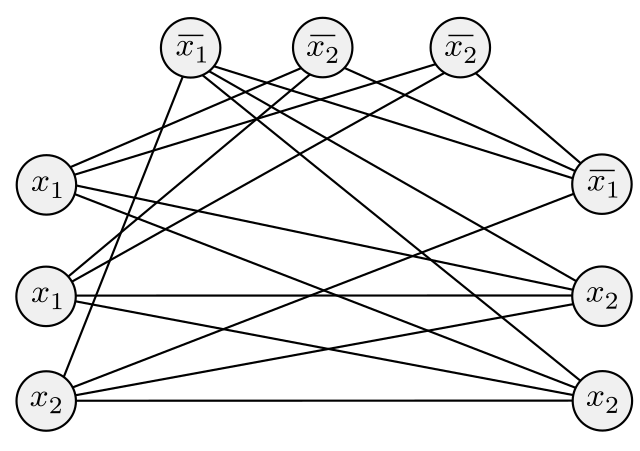
\includegraphics[scale=0.5]{figur/figur733.png}
	\end{center}

	Denne kommer fra formlen $\phi = (x_{1} \vee x_{1} \vee x_{2}) \wedge (\overline{x_{1}} \vee \overline{x_{2}} \vee \overline{x_{2}}) \wedge (\overline{x_{1}} \vee x_{2} \vee x_{2})$.

	Bemærk her at der er kanter mellem to knuder hvis:
	\begin{enumerate}
		\item De \textbf{ikke} er i klausul sammen
		\item De \textbf{ikke} er omvendte af hinanden ($x_{i}$ og $\overline{x_{i}}$)
	\end{enumerate}
	Vi påstår at hvis hver literal i en klikke evalueres til at være sand, så er det en sand sanhedsfordeling. For eksempel, i dette eksempel er $\overline{x_{1}}, x_{2}, x_{2}$ en klikke, og ved at lade disse evalueres til sand får vi en sand formel. Hvis $x_{1} = F$ så er $\overline{x_{1}} = T$ og $x_{2}$ er blot sand i begge tilfælde.

	Vi kan beskrive kanternes konstruktion som følger:
	\begin{equation*}
		E(G) = \{v_{i,j} v_{i',j'} \mid i \ne i' \text{ og } \lambda_{i_{j}} \ne \overline{\lambda_{i'_{j'}}}\}
	\end{equation*}

	\begin{claim}
		$G$ har en $k$-klikke $\iff$ $f$ er satisfiable.
	\end{claim}

	\begin{proof}
		\(\Rightarrow\):\\
		\noindent
		Lad $H$ være en $k$-klikke  i $G$. Så
		\begin{itemize}
			\item $|H \cap \{v_{i,{1}}, v_{i,2}, v_{i_{3}}\}| = 1 \forall i \in \{1, 2, \ldots, k\}$
			\item Hvis en knude $x_{j}$ er i $H$ så er der ingen knude $\overline{x_{j}}$ i $H$ .
		\end{itemize}
		Lad:
		\begin{equation*}
			\phi(x_{i}) = \begin{cases}
				T \text{ hvis  en knude af H er kaldt} x_{i} \\
				F \text{ hvis en knude af H er kaldt } \overline{x_{i}} \text{ eller ingen knude i H kaldes } x_{i} \text{ eller }  \overline{x_{i}}
			\end{cases}
		\end{equation*}
		\(\Leftarrow\): \\
		\noindent
		Antag $p : \{x_{1}, x_{2}, \ldots, x_{n}\} \rightarrow \{T, F\}^{n}$ satisfier $f$:
		\begin{itemize}
			\item Vælg en sand literal \(\lambda_{i_{j}}\) i $c_{i}$ for $i = 1, 2, \ldots, k$
			\item For $i := 1$ til $k$. Put knuden skrevet $\lambda_{ij}$ i $H$
			\item $H$ er en $k$-klikke
		\end{itemize}
	\end{proof}
	Dermed, given $f$ kan vi konstruere $\langle G, k \rangle$ i tid $O(|f|^{2})$.
\end{proof}

\subsection{CLIQUE $\le_{p}$ Independent Set}%
\label{subsec:label}



\begin{definition}[Komplement af en graf]
	\textit{Komplemented} af en graf $G = (V, E)$ er en graf $\overline{G} = (V, \overline{E})$ som indeholder alle de knuder der ikke var i $G$, men ingen af de knuder der var i $G$, altså $(u,v) \in \overline{E} \iff (u,v) \notin E$.
\end{definition}
Bemærk ud fra denne definition at $(V, E \cup \overline{E})$ giver en komplet graf.

\begin{definition}[Uafhængig delmængde]
	Lad $G = (V,E)$ være en graf. En delmængde $W \subseteq V$ er \textit{uafhængig} hvis ingen kant $(u,v) \in E$ har $|\{u,v\} \cap W| = 2$
\end{definition}

Altså vil det sige at for hver to knuder i en uafhængig mængde er der ingen kanter mellem dem, trods der muligvis ville være i $V$.

Vi opstiller nu problemet \textit{Uafhængig Mængde} (på engelsk Independent Set, forkortet IS): Given en graf $G = (V,E)$ og $q \in \mathbb{Z}_{+}$, har $G$ en uafhængig mængde af størrelse $q$?

\begin{theorem}
	Independent Set \(\in \mathcal{NPC}\)
\end{theorem}

\begin{proof}
	Vi viser først et certifikat, så en reduktion.
	\begin{enumerate}
		\item Certifikatet er en mængde af knuder, som ingen kanter har mellem sig.
		\item CLIQUE $\le_{p}$ IS:
	\end{enumerate}
	$X$ er en klikke i $G \iff X$  er en uafhængig mængde i $\overline{G}$. \(\langle G, k \rangle \in\) CLIQUE $\iff$ \(\langle \overline{G}, k \rangle \in\) uafhængig mængde. Vi laver en polynomiel reduktion.
\end{proof}

\subsection{Independent Set $\le_{p}$ Vertex-Cover}%
\label{subsec:label}

\begin{definition}
	Et \textit{vertex cover} i en graf $G = (V,E)$ er en delmængde $U \subseteq V$ hvor $|\{u,v\} \cap U| \ge 1 \; \forall (u,v) \in E$.
\end{definition}

Vertex-Cover problemet siger: Given en graf $G = (V,E)$ og $p \in \mathbb{Z}_{+}$, har $G$ en dækning af knuder af størrelse $p$?

\begin{theorem}
	Vertex-Cover $\in \mathcal{NPC}$
\end{theorem}
\begin{proof}
	Vi viser først et certifikat og så reduktion.
	\begin{enumerate}
		\item Certifikatet er en mængde $U \subseteq V$ hvor, hvis man fjerne $U$ så fjerner det \textit{alle} kanterne.
		\item Independent Set $\le_{p}$ Vertex-Cover
	\end{enumerate}
	$X$ er uafhængigt i $G$ $\iff$ $V \setminus X$ er en dækning af knuder i $\overline{G}$. Dermed \(\langle G, q \rangle \in \) Independent Set $\iff$ \(\langle \overline{G}, |V(G)| - q \rangle \in \) Vertex-Cover.
\end{proof}


\subsection{3-SAT $\le_{p}$ Vertex-Cover}%
\label{subsec:label}

Vi har allerede set SAT $\le_{p}$ 3-SAT $\le_{p}$ Clique $\le_{p}$ Independent Set $\le_{p}$ Vertex-Cover. Her giver vi en direkte reduktion 3-SAT $\le_{p}$ Vertex-Cover.

Givet en instans $f = C_{1} \wedge C_{2} \wedge \ldots \wedge C_{m}$ af 3-SAT med variablerne $x_{1}, x_{2}, \ldots, x_{n}$:
\begin{itemize}
	\item Lad $k = n + 2m$ og konstruer en graf $G = G(f')$ med $2n+3m$ knuder.
	      \begin{itemize}
		      \item Hver variabel $x_{i}$ repræsenteres af $(v_{i}, \overline{v_{i}})$ i $G$
		      \item Hver klausul $c_{j}$ repræsenteres af
	      \end{itemize}
\end{itemize}






%%% Local Variables:
%%% mode: latex
%%% TeX-engine: xetex
%%% TeX-command-extra-options: "-shell-escape"
%%% TeX-master: "main"
%%% End:
